\begin{figure}[hbtp]
  \centering
  \subfigure{
    \label{fig:adjust-auxiliary--8020}
    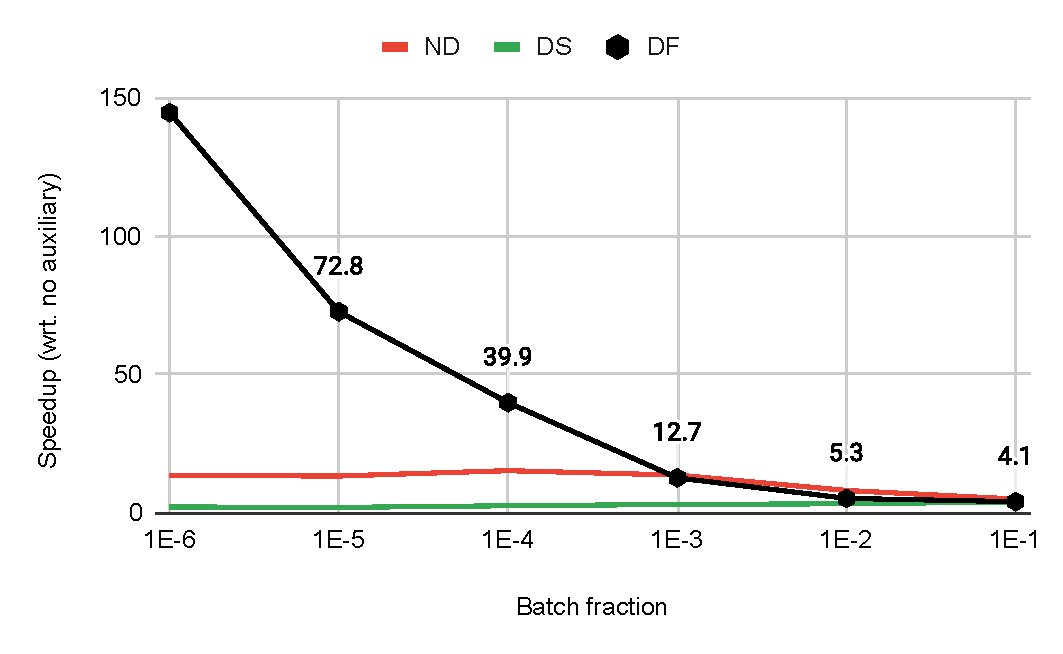
\includegraphics[width=0.98\linewidth]{out/adjust-auxiliary-8020.pdf}
  } \\[-2ex]
  \caption{Speedup of \textit{Naive-dynamic (ND)}, \textit{Delta-screening (DS)}, and \textit{Dynamic Frontier (DF)} Louvain when reusing the previous \textit{weighted-degrees of vertices} and \textit{total edge weight of communities} as auxiliary information to the dynamic algorithm, compared to the same dynamic algorithm when both are recomputed from scratch. This is done on large graphs with generated random batch updates of size $10^{-7} |E|$ to $0.1 |E|$\ignore{, consisting of $80\%$ edge insertions and $20\%$ deletions, to simulate realistic dynamic graph updates}.}
  \label{fig:adjust-auxiliary}
\end{figure}
